% -----------------------------------------------------------------------------

%Reference corpus compilers and those carrying out linguistic studies 
% i've removed narrow focus on 'domain-specific' in the following
Those using corpus data are increasingly turning
to the web as a source of language data. 
This is not surprising given the vast quantities of downloadable data
that are readily available online. 
The Web as Corpus (WaC) paradigm\cite{kilgarriff2003introduction} 
has become popular for compilers of corpora for lexicographic use, 
replication of standard reference corpora as well as for studies of specific online varieties of language. 

Two general models of WaC have emerged. Using the first model, `browsing', corpus compilers collect data from a set of given domains and select whole or part texts online and incorporate them into their corpora (e.g. the BE06\cite{baker2009be06} corpus comprising material published in paper form but found on the web).
%This is the model used for compilation of new reference corpora, e.g. BE06\cite{baker2009be06} containing material previously published in paper form but found on the web. 

The second model, `searching', sees the web through the lens of search engines, and is typically used to compile domain-specific corpora from a set of seed terms which are used to locate web pages for incorporation into a corpus (e.g. the BootCat \& WebBootCat tools \cite{baroni2004bootcat}). % THAT OR WHICH 
% which is ok, see: http://www.oup.com/uk/booksites/content/0199296251/essentials/grammartips/
%This approach is embodied in the BootCat and WebBootCat tools.
In some cases, both approaches are combined, using searching for general language seed terms to produce reference corpora\cite{kilgarriff2010corpus}.

% --------- overview of WAC ----------
%These two WaC approaches can be seen as taking a snapshot of online data.  % TODO: moved to the data section
Collecting corpora online raises legal questions regarding redistribution rights.  Consequently, many compilers choose to make data available only through a web interface (with restricted access for fair-use) or by distributing URI lists (known as open-source corpora\cite{sharoff2006open}).



%If a corpus is collected online, then the legal grey area of redistribution rights means that many compilers chose to make data available only through a web interface (with restricted access for fair-use) or by distributing URI lists, known as open-source corpora \cite{sharoff2006open}.
Online content changes much faster due to the decentralised, open publishing model of the web, which may have a serious impact on two aspects of the WaC paradigm: availability and replicability.

If websites change, the URI lists need updating to reflect new locations. 
Worse, websites or pages may be completely removed, thus the corresponding part of a corpus is no longer available.
This attrition of documents through time affects both users of open-source corpora 
and those attempting to interpret the results of studies using corpora that were built just a few years ago.

\subsection{Background}
% ------- background -------
% TODO: mention document attrition
Though many studies have looked at the life-cycle of web pages in general, these typically focus on the integrity of websites or specific repositories of information, rather than the documents and the language contained within.



\cite{koehler2002web}, through four years of weekly sampling, found that just 66\% of their original seed URIs remain online after a year, with this proportion dropping to around 31\% by the end of the study.  Koehler started his study in the early days of the web (December 1996) using a relatively small sample of only 361 URIs.  His analysis found differences in the type of page as well as variation across top-level domains (TLD). %that sentence sucks; study such as cho2000evolution again... i've fixed this to some extent
% I'd need to see the Koehler study but I could style this paper as an update of Koehler's work on a much larger scale and with a corpus focus?

\cite{nelson2002object} found that only 3\% of documents in digital libraries become unavailable in just over a year. This is perhaps unsurprising given the aim of such projects but serves to illustrate the degree of heterogeneity between types of document host.  
% do you mean 'unavailable'?

%Bar-Ilan and Peritz \cite{bar1999life} present a slightly different method of study, searching for the same information where URIs became unavailable.  Though they primarily investigate the growth of the web in their analysis of the availability of information, they find a similar amount of na\"{i}ve URI attrition to the above studies after a year. % TODO: change to names!


% this is irrelevant, but studied in their study:  Due to the growth of the web, their relatively technical subject matter (often hosted on sites seen in other studies to be more long-lived), and sampling method, they find that information online is often available more readily than the naive URI death-time would suggest % ahrg, terribly written ;-)

% I think this is probably irrelevant [Though focusing on mapping sites in their entirety, a more thorough effort to model loss by content type is made by Cho and Garcia-Molina \cite{cho2000evolution}, who develop a model to optimise site crawling, with the aim being to maximise availability for other search engines.]


% ------ academic ref section?
Studies involving academic paper availability mirror open source corpora in that they use references in favour of original text, however, the centralised administration of academic repositories is notably in contrast to most web resources.  Nevertheless, there has been much work into this area, some of which is comparatively reviewed in a paper by \cite{sanderson2011analyzing}.  These studies, spanning years from 1993 to 2008, illustrate that even institutions charged with keeping an accessible record of information are still subject to rates of attrition in the region of 25-45\% over five years.

% ------ /academic refs


Despite these enquiries, very little work has been carried out to estimate the effects that document attrition has upon corpus content.  %, (or vice versa, technically). 
% I could extend that vice-versa in the full paper, nice idea!
\cite{sharoff2006creating} touches upon this in his WaC work , presenting a preliminary analysis of attrition within corpora generated by searching for 4-tuples.  Although his studies lasted from one to five months, and contained modest sample sizes (1000), they indicate a rate of loss that is below that of other studies (just 20\% per year in the month-long study), suggesting that the selection of documents may have significant effects upon document attrition rates.
% i think this is what you meant?


% ---------- What I're doing ----------
%Very little work has been carried out to estimate the effects of this skew on corpora built using web data
%Sharoff \cite{sharoff2006creating}
%calls this `URI half-life' and tries to estimate the rate of disappearance of URIs in his corpus.
%In this paper, I use the term `document attrition'. I outline a preliminary analysis of this skew,
%attempting to identify trends within corpora of differing construction. I use a number of corpora
%and present results over a short time period to determine the scale of the problem. This paper is part of
%a longer term study which will compare other features such as text type and features of the websites
%such as academic/commercial, country, etc. %  need to beef this up --- is this sufficiently beefed? I fear I've beefed the wrong bit [23-10]


Rather than analysing web resources in isolation of their linguistic uses, I outline a preliminary analysis of what I term `document attrition' relative to a number of corpora of differing construction.  I do this by comparing each corpus' construction with a series of URI-based explanatory variables, as part of a larger longitudinal study that will go on to use full text features in order to identify linguistic influence and trends upon web-based corpora and document attrition as a whole.


%In this paper I present a preliminary analysis of online document attrition relative to URI-based explanatory variables
%% give a couple of examples in brackets?
%, in an attempt to gauge the influence these variables have upon the corpora used.  

%%The URI features analysed in this paper are selected to be indicative of document content, publisher status, or purpose, and are designed to complement further longitudinal studies performed using full-text features using this data set. % ack, very ugly, try: -- I concur :-)
%This paper is part of a larger longitudinal study that will go on to use full text features in order to identify linguistic influence and trends upon web-based corpora and document attrition as a whole.


% looks good so far

% ------------- Vestigial notes -----------
% corpora built on different dates technically mandate different analysis periods, so short-term is a bit of a misleading statement.
% omit this in the extended abstract for space reasons
% Start with a brief review of the literature surrounding WaC as well as some efforts to quantify the document attrition problem, go 
% on to look at the process used by others (and adapted by us) for sampling these documents continue to present preliminary results, 
% analysing a subset of the downloaded data in a longitudinal fashion Conclude with a brief summary of hitherto indicated trends and 
% a discussion of what work lays before us on the winding yellow road of science.




% -----------------------------------------------------------------------------




% ####### Datamethods.tex

\subsection{Methods \& Data}


% ----------- What I'm doing ----------
In order to measure document attrition across a number of linguistic sources I selected a series of corpora, chosen due to their differing constructions and ages, and downloaded them using a process that closely approximates an end user's view of the web.  Statistics on the availability of these documents were then annotated with a series of URI-related variables for analysis.




\subsubsection{Data Summary}
Data were taken from four open-source corpora (outlined in Table \ref{table:datmeth:datasum}), each of which consist of a sample of URIs referring to web resources.  All of these corpora are cross-sectional, representing data from a short period, however, only the BootCat-based corpora are built using a script that is likely to sample quickly enough to count as a true point sample in the context of this study.

%\{I want to float table 1 on THIS page, but LaTeX isn't playing}
\begin{table*}[ht!]
    \centering
    \begin{tabular}{r | r | r | r | l  }
    Corpus    & Date	    & Size (URIs)   & Sample Period	& Construction \\ 
    \hline
    BE06      & 2006	    & 473	    & 1 year		&  Browsing \\ 
    Delicious & Sep. 2009   & 630,476	    & 1 month		&  Browsing \\
    Sharoff   & 2006\footnote{Sharoff does not state which month this sample was taken, it is presumed to be June}	    
                            & 82,257	    & hours		&  Searching \\
    BootCat  & Sep. 2011   & 177,145	    & hours		&  Searching \\ 
    \end{tabular}

    \caption{An overview of the corpora selected for study.}
    \label{table:datmeth:datasum}
\end{table*}

BE06 %\cite{baker2009be06} 
was built as a conventional, hand-selected corpus designed as an update to the LOB\cite{johansson1980lob} and FLOB\cite{hundt1998manual} corpora.  It contains texts from sources published in 2006 but also available online.

The Delicious corpus represents a sample of links posted to the front page of delicious.com\footnote{A social bookmarking site where users post and exchange links.} during the whole of September 2009.  

Sharoff's corpus is the same one used in his 2006 paper on open-source corpora, and is built using modified BootCat scripts from a series of 4-tuple seed terms selected from the British National Corpus.

The BootCat corpus is built for this study from 4-tuples that are themselves built from the same terms as Sharoff uses for his 2006 study, using updated versions of his original scripts\footnote{As published online at \\ \url{http://corpus.leeds.ac.uk/internet.html}}.


%Corpora were sampled at the same points in time... see tex notes %[the assumption implicit in this is that the drift is regular, however, this can be tested by not comparing analyses]
%For the purposes of this study, no text content from the links themselves were analysed, meaning that sites incorrectly reporting failure through web-based handlers appear as silent non-failed links.


% -----------------------------------------------------------------------------
% * Format of the data (http, raw, headers, did I use text or just request properties?)
% * Representativeness issues addressed by use of corpora from different creative causes (be06, google, delicious)
% * Brief Summaries of data % IF there's space!









\subsubsection{Downloading Process}
The process of recording the document's status was relatively simple: a small piece of custom software was written to download documents from an open-source corpus at regular intervals.  This tool was configured to mimic requests made by common web browsing software in order to emulate a typical user's visit to the document. Handling SSL, cookies, and referrer links in a similar manner to a user following a bookmark allows us to assess more accurately the content, avoiding tricks that exploit search engine crawlers and other bots.


%Since the aim is to emulate a typical web visitor, this downloading process must emulate common web browsing software, and request documents using relatively ordinary HTTP request parameters.  This aspect of our method is perhaps slightly uncommon: many corpus building efforts do not pain themselves to handle features such as HTTPS or cookies, and many do not spoof the referrer or user-agent request strings.

% HTTPS, cookies accepted
% spoofs as firefox on windows XP


Taking this user perspective, the notion of document availability becomes slightly more complex.  Redirect requests were followed up to a depth of 5\footnote{As recommended in the HTTP specification and commonly implemented in browsers}.  Since I do not account for content changing in this study, failure was taken as receiving a HTTP status code other than 200, or a network timeout (60 seconds was the timeout used for DNS and TCP)%
\footnote{Timeout errors also occur stochastically due to routing policies, and are impossible to avoid entirely when downloading resources in bulk.  The download process was tuned to minimise this source of error.}.

%In accordance with this emulation of a typical user, the point at which documents become unavailable should also be clarified.  A lack of availability is most likely to manifest itself as a removal of the desired content (aside from, say, a mere change of site design or name), presenting a few ways in which this may technically manifest:

%\begin{itemize}
    %\item HTTP status codes other than 200;
    %\item DNS or TCP timeouts --- these indicate that a host has been moved or made unavailable.
    %%those codes which indicate a failure to locate (4xx) or render (5xx) content are cause to assume the website has taken content down;
    %\item DNS lookup timeouts --- Indicating that a user has closed or moved their domain;
    %\item TCP timeouts        --- Indicating that the host is down.  Occasionally, timeouts will be due to a temporary network error\footnote{These errors occur stochastically due to routing policies, and are impossible to avoid entirely when downloading resources in bulk.}, and samples which fail a single time should be filtered out (providing their content remains static).
    %%of the 10-30 seconds it is commonly said people will await page loading\cite{king2003optimisation}. % http://www.websiteoptimization.com/speed/1/ 
%\end{itemize}

%Both TCP and DNS timeouts were set to 60 seconds for this study.

% mention spoofing in detail? this section seems to end abruptly
%  > probably keep any more detail for the full paper later

% ---- data source and type
Both metadata and original response details are stored by the download software.  This study will focus on features of URIs, such as the presence of GET arguments\footnote{Parameters appended to a URI string, typically used to control dynamic scripts}
in the URI string, meaning that the resource is likely to be dynamic.  These features have been chosen to indicate aspects of web hosting and affiliation that are likely to vary between users with both different reasons for uploading their content, and different degrees of technical expertise.


%The variables identified are summarised in table [
%], along with the reason for their selection.

%VARIABLES
%link_id       effectiveuri  duration      uri_tld       uri_frag
%sample_id     errorcode     complete      uri_sld       uri_fraglen
%rtt           id            errors        uri_hld       uri_len
%rdt           c200          uri           uri_npath     
%dnst          c404          disabled      uri_pathlen   
%encoding      cother        uri_valid     uri_querylen  
%responsecode  datetime      uri_scheme    uri_nargs     

% all looks good down to here


% -----------------------------------------------------------------------------
% * Acquire massive list of URIs (open source corpus)
%   - bootcat
%   - manually built
%   - Delicious
%   (*** depending on quality of data, make a thing of the comparison or not)
% * Time-series data samples using custom software
% * Record loss, response times, etc
%---
% * What constitutes 'death' (404, 504, 503, !200, timeout, change, etc)
% * What covariates are used (see url analysis script and add some from the db)
% * Explain roughly some expectations from observation, ie n\%/day
% * Download method, relate to bootcat/serge
%40 pages about swearing at cron

% -----------------------------------------------------------------------------







\subsection{Results}



% for the extended abstract, I'd suggest a couple of table with descriptive stats to get the point across
% -----------------------------------------------------------------------------


Table \ref{table:longitudinal:attrition-inputdist} describes the availability of documents within the corpora, as sampled on the 21st October 2011.  This forms two data points, the former representing no attrition when the corpus was first compiled.  
Document lifetime statistics are calculated assuming exponential decay: both the half-life ($t_{1/2}$, the time it takes for only half of the original corpus to remain available) and the mean lifetime, $\tau$, are provided.



%Taking the most permissive definition of a document being unavailable, (websites returning status codes other than 200) the raw loss observed in the single most recent sample, taken , may be seen in table \ref{table:res:loss}.


% LOSS PERCENTAGES
    %> summary(be.s3$non200)
       %Mode   FALSE    TRUE    NA's 
    %logical     268     197       0 
    %> 197/473
    %[1] 0.4164905
    %> summary(deli.s3$non200)
       %Mode   FALSE    TRUE    NA's 
    %logical  581033   47365       0 
    %> 47365/630476
    %[1] 0.07512578
    %> summary(serge.s3$non200)
       %Mode   FALSE    TRUE    NA's 
    %logical   53559   28351       0 
    %> 28351/82257
    %[1] 0.3446637
    %> summary(boot.s3$non200)
       %Mode   FALSE    TRUE    NA's 
    %logical  174993    1445       0 
    %> 1445/177145
    %[1] 0.008157159
% HALF-LIVES
    %> halflife(473, 268, 1954)
    %[1] 2384.069
    %> halflife(630476, 581033, 766)
    %[1] 6501.368
    %> halflife(82257, 53559, 1954)
    %[1] 3156.656
    %> halflife(177145, 174993, 31)
    %[1] 1758.014



\begin{table}[h*tb]
    \centering
    \begin{tabular}{r | r | r | r | l}
	  Corpus & Age (yr.) & Loss & $t_{1/2}$ (yr.) & $\tau$ (yr.) \\
	\hline 
	
	%BE06       & 5.3 / 1954 & 42\%    & 6.53 / 2384\\
	%Delicious  & 2.1 / 766  & 7\%	  & 17.81 / 6501\\
	%Sharoff    & 5.3 / 1954 & 34\%    & 8.64 / 3156\\
	%BootCat   & .08 / 31   & 0.8\%   & 4.84 / 1758\\
	BE06       & 5.3  & 42\%    & 6.5	& 15.8\\
	Delicious  & 2.1  & 7\%	    & 17.8 & 42.4\\
	Sharoff    & 5.3  & 34\%    & 8.6  & 16.4\\
	BootCat    & .08  & 0.8\%   & 4.8  & 20.4\\
    \end{tabular}

    \caption{Loss from corpus inception to October 21st, 2011.}
    \label{table:longitudinal:attrition-inputdist}
\end{table}

% ---- Rate of failure per corpus
The large differences in corpus half-life are revealing --- the Delicious corpus has significantly lower loss than the others.  This is ostensibly owing to its construction: users are likely to bookmark resources that are useful (and hence are well-established, popular sites), in contrast to BootCat's uncritical selection or the deliberate {\it document}-seeking (rather than {\it information}-seeking) represented by BE06.


% ---- Differences between cats
The difference in half-life between Sharoff's corpus and our own BootCat-derived one is harder to explain.  Though both are large corpora built using similar methods, they were sampled years apart with heavy influence from search engines (which will have updated significantly in this period).  It is also possible that 31 days is an insufficient period to achieve an estimate for attrition that is representative of a full year's loss, implying that a pattern may be evident due to external influences (such as hosting renewals around the commencement of the tax year).%, a point to be addressed in our planned high-resolution longitudinal study.
% TODO: talk about plans in conclusion


% --- half-life comparison to koehler
Although I have omitted an analysis of content here, the half-lives of our samples are above those stated in other, more general, studies (Koehler reports a half-life of 2.4 years, for example).
This may be the result of bias introduced when deliberately omitting non-document portions of the web, such as navigation pages or images.  Another influence is the age of many attrition studies, as it is possible that, with reduction in the price of web hosting, resources simply remain online for longer.
%Although I have omitted an analysis of content here, all of the above figures indicate half-lives above those found in other papers.  The extent to which this is explainable by deliberate bias in corpus sampling (selecting documents rather than pictures, navigational pages etc.) is unclear, since I lack a sample taken from a crawler. % (probably a TODO, to be compared to others, but the crawler would matter a lot...).


% ---- Why has be06 dropped so fast?
The relatively high rate of attrition in BE06 is surprising given that it only features documents that were already in print, which ostensibly reside in archives or the websites of large institutions (shown to be relatively nonvolatile in other work).  One possible counter argument is that BE06's sampling policy was to take documents {\it published} in 2006, rather than merely being available, such that these samples have witnessed the initial steep descent on the document survival curve. %this explanation does nothing to explain the short half-life of the younger BootCat though!

% might it be that these docs are still available, but moved to a new location with no URL redirect in place? so they are still available by 'searching' but not 'browsing'? This might indicate a new methodology for distributing URI lists?

% HTTP error codes per corpus
    %> summary(factor(be.s3$responsecode))
    %200 400 404 500 503 504 
    %268  25 160   2   2   8 
    %> summary(factor(deli.s3$responsecode))
	 %0    200    204    300    301    302    303    307    400    401    402 
	 %2 581033      8     54     25     10      1      3    973    203      5 
       %403    404    405    406    408    409    410    414    415    423    500 
      %1411  30386      9      4      2      2    565      1     12      7   1279 
       %501    502    503    504    505    510    999 
	 %1    349   8394   3656      1      1      1 
    %> summary(factor(serge.s3$responsecode))
      %200   204   300   301   302   400   401   402   403   404   405   406   408 
    %53559     4    30    15     7   176    75     3   320 22609     2     3     1 
      %409   410   415   417   500   502   503   504 
	%1   301    52     1   373    90  3037  1251 
    %> summary(factor(boot.s3$responsecode))
       %200    400    401    403    404    408    410    500    502    503    504 
    %174993     12      2     64    691      1     15     92     10    349    209 
% ---- HTTP status codes
The diversity of status codes returned varies significantly between corpora, with older ones showing more intricate and descriptive modes of failure (such as code \texttt{410 Gone}).  Delicious exhibits differences to the other corpora, exhibiting codes that are presented by WebDAV and similar systems unlikely to be crawled by search engines.% (code \texttt{423}, \texttt{300}, \texttt{405}, \texttt{407}) unlikely to be spidered by search engines.


% PER-TLD
	%Pearson's Chi-squared test

%data:  table(t1$non200, t1$simpletld) 
%X-squared = 33.8761, df = 6, p-value = 7.108e-06

%Warning message:
%In chisq.test(table(t1$non200, t1$simpletld)) :
  %Chi-squared approximation may be incorrect
%> testTLD(deli.s3)

	%Pearson's Chi-squared test

%data:  table(t1$non200, t1$simpletld) 
%X-squared = 1348.946, df = 7, p-value < 2.2e-16

%> testTLD(boot.s3)

	%Pearson's Chi-squared test

%data:  table(t1$non200, t1$simpletld) 
%X-squared = 340.7064, df = 7, p-value < 2.2e-16

%Warning message:
%In chisq.test(table(t1$non200, t1$simpletld)) :
  %Chi-squared approximation may be incorrect
%> testTLD(serge.s3)

	%Pearson's Chi-squared test

%data:  table(t1$non200, t1$simpletld) 
%X-squared = 1243.207, df = 7, p-value < 2.2e-16



%--------------------------------------------------------------------------------

%> be.s3$simpletld = mapply( simplifyTLD, be.s3$uri_tld )
%> be.tld.glm.logit = glm( factor(non200) ~ factor(simpletld), family=binomial(), data=be.s3)
%> summary(be.tld.glm.logit)

%Call:
%glm(formula = factor(non200) ~ factor(simpletld), family = binomial(), 
    %data = be.s3)

%Deviance Residuals: 
   %Min      1Q  Median      3Q     Max  
%-1.482  -1.011  -0.535   1.131   2.007  

%Coefficients:
                       %Estimate Std. Error z value Pr(>|z|)    
%(Intercept)             -0.4055     0.1543  -2.628 0.008596 ** 
%factor(simpletld)edu   -14.1606   882.7434  -0.016 0.987201    
%factor(simpletld)info  -14.1606   624.1938  -0.023 0.981901    
%factor(simpletld)net     1.0986     1.2344   0.890 0.373478    
%factor(simpletld)org    -1.4663     0.4099  -3.577 0.000347 ***
%factor(simpletld)other  -0.2877     0.8797  -0.327 0.743641    
%factor(simpletld)uk      0.5157     0.2055   2.510 0.012079 *  
%---
%Signif. codes:  0 ‘***’ 0.001 ‘**’ 0.01 ‘*’ 0.05 ‘.’ 0.1 ‘ ’ 1 

%(Dispersion parameter for binomial family taken to be 1)

    %Null deviance: 633.74  on 464  degrees of freedom
%Residual deviance: 595.68  on 458  degrees of freedom
%AIC: 609.68

%Number of Fisher Scoring iterations: 13


%--------------------------------------------------------------------------------



%> deli.s3$simpletld = mapply( simplifyTLD, deli.s3$uri_tld )
%> deli.tld.glm.logit = glm( factor(non200) ~ factor(simpletld), family=binomial(), data=deli.s3)
%> summary(deli.tld.glm.logit)

%Call:
%glm(formula = factor(non200) ~ factor(simpletld), family = binomial(), 
    %data = deli.s3)

%Deviance Residuals: 
    %Min       1Q   Median       3Q      Max  
%-0.4909  -0.3881  -0.3769  -0.3769   2.3153  

%Coefficients:
                        %Estimate Std. Error  z value Pr(>|z|)    
%(Intercept)            -2.609253   0.006366 -409.879  < 2e-16 ***
%factor(simpletld)edu    0.553917   0.028144   19.682  < 2e-16 ***
%factor(simpletld)gov    0.292298   0.049494    5.906 3.51e-09 ***
%factor(simpletld)info   0.362535   0.056889    6.373 1.86e-10 ***
%factor(simpletld)net    0.104815   0.020799    5.039 4.67e-07 ***
%factor(simpletld)org    0.061073   0.015354    3.978 6.96e-05 ***
%factor(simpletld)other  0.412508   0.012910   31.952  < 2e-16 ***
%factor(simpletld)uk     0.121198   0.027791    4.361 1.29e-05 ***
%---
%Signif. codes:  0 ‘***’ 0.001 ‘**’ 0.01 ‘*’ 0.05 ‘.’ 0.1 ‘ ’ 1 

%(Dispersion parameter for binomial family taken to be 1)

    %Null deviance: 335971  on 628397  degrees of freedom
%Residual deviance: 334718  on 628390  degrees of freedom
%AIC: 334734

%Number of Fisher Scoring iterations: 5




%--------------------------------------------------------------------------------


%> boot.s3$simpletld = mapply( simplifyTLD, boot.s3$uri_tld )
%> boot.tld.glm.logit = glm( factor(non200) ~ factor(simpletld), family=binomial(), data=boot.s3
%+ )
%> summary(boot.tld.glm.logit)

%Call:
%glm(formula = factor(non200) ~ factor(simpletld), family = binomial(), 
    %data = boot.s3)

%Deviance Residuals: 
    %Min       1Q   Median       3Q      Max  
%-0.2265  -0.1195  -0.1195  -0.1137   3.2151  

%Coefficients:
                       %Estimate Std. Error  z value Pr(>|z|)    
%(Intercept)            -4.93882    0.03732 -132.339  < 2e-16 ***
%factor(simpletld)edu    0.18271    0.12182    1.500    0.134    
%factor(simpletld)gov    1.28831    0.08422   15.297  < 2e-16 ***
%factor(simpletld)info  -0.22406    0.57998   -0.386    0.699    
%factor(simpletld)net    0.05991    0.16114    0.372    0.710    
%factor(simpletld)org   -0.09896    0.07724   -1.281    0.200    
%factor(simpletld)other  0.73659    0.09135    8.063 7.42e-16 ***
%factor(simpletld)uk    -0.10358    0.13800   -0.751    0.453    
%---
%Signif. codes:  0 ‘***’ 0.001 ‘**’ 0.01 ‘*’ 0.05 ‘.’ 0.1 ‘ ’ 1 

%(Dispersion parameter for binomial family taken to be 1)

    %Null deviance: 16764  on 176437  degrees of freedom
%Residual deviance: 16523  on 176430  degrees of freedom
%AIC: 16539

%Number of Fisher Scoring iterations: 7


%--------------------------------------------------------------------------------

%> serge.s3$simpletld = mapply( simplifyTLD, serge.s3$uri_tld )
%> serge.tld.glm.logit = glm( factor(non200) ~ factor(simpletld),family=binomial(), data=serge.s3
%+ )
%> summary(serge.tld.glm.logit)

%Call:
%glm(formula = factor(non200) ~ factor(simpletld), family = binomial(), 
    %data = serge.s3)

%Deviance Residuals: 
    %Min       1Q   Median       3Q      Max  
%-1.1172  -0.9445  -0.8343   1.3957   1.5694  

%Coefficients:
                        %Estimate Std. Error z value Pr(>|z|)    
%(Intercept)            -0.876551   0.011039 -79.406  < 2e-16 ***
%factor(simpletld)edu    0.484895   0.029115  16.654  < 2e-16 ***
%factor(simpletld)gov    0.611879   0.041594  14.711  < 2e-16 ***
%factor(simpletld)info  -0.009887   0.144528  -0.068    0.945    
%factor(simpletld)net    0.311257   0.038870   8.008 1.17e-15 ***
%factor(simpletld)org    0.300543   0.020496  14.663  < 2e-16 ***
%factor(simpletld)other  0.733223   0.023990  30.563  < 2e-16 ***
%factor(simpletld)uk     0.376607   0.026484  14.220  < 2e-16 ***
%---
%Signif. codes:  0 ‘***’ 0.001 ‘**’ 0.01 ‘*’ 0.05 ‘.’ 0.1 ‘ ’ 1 

%(Dispersion parameter for binomial family taken to be 1)

    %Null deviance: 105666  on 81909  degrees of freedom
%Residual deviance: 104438  on 81902  degrees of freedom
%AIC: 104454

%Number of Fisher Scoring iterations: 4


%--------------------------------------------------------------------------------



% TLD rates (not statistically rigorous, just a quick eyeball)

\begin{figure}[Ht]
    \centering
    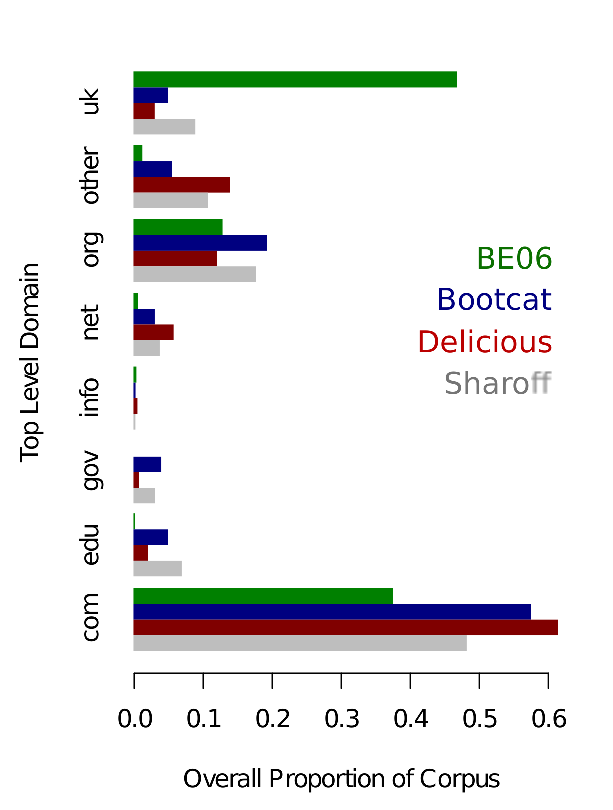
\includegraphics[width=0.6\textwidth]{longitudinal/attrition-all-tlds}
    \caption{Overall distribution of top level domains.}
    \label{fig:longitudinal:attrition:attrition-all-tlds}
\end{figure}





Each of the corpora exhibit similar distributions of each top level domain (TLD), though the large differences in sample size make formal comparison difficult.  The overall distribution of the more popular domains is provided in Figure \ref{fig:longitudinal:attrition:attrition-all-tlds}.  This indicates that \texttt{.com} dominates the selection across corpora, with \texttt{.org} following.  Only BE06 differs from this distribution in its selection of \texttt{.uk} addresses, however, it has been deliberately biased this way so as to represent British English.


Other studies have identified statistically significant differences in the rate of attrition between the major TLDs.  
Though each corpus exhibits a dependence between these TLD groups (chosen to represent the vast majority of each corpus' content) in a $\chi^2$ indepdence test ($\chi^2 > 33.8; p<0.01$ in all cases), generalised linear models reveal that the nature of this dependence varies greatly between corpora, indicating that this estimate is far too simplistic to represent the real causes of attrition.


%a more detailed model does not display any reveal significant differences between those identified in other studies.  For each of the four sample corpora, \texttt{.edu}, \texttt{.info} and \texttt{.org} display similar rates of attrition to \texttt{.com} and \texttt{.uk}.  It seems reasonable to conclude that this effect is as a result of the low frequency of certain more obscure TLDs such as \texttt{.tv}, many of which are revealed to be significant when predicting loss for each corpus using a logistic regression model.




%In accordance with other studies on more general-purpose web content, there are minor observable differences between TLD longevity, with \texttt{.edu}, \texttt{.info} and \texttt{.org} displaying lower rates of attrition overally than \texttt{.com} or \texttt{.uk}.  
%These differences are not statistically significant, however, for any of the corpora used.


% TODO, possibly graphs.  This would be nice to cut if I run out of space since it's only confirmatory and there are few patterns between the corpora














%t URI PATH LENGTH
    %> plot(  density(be.s3$uri_npath)  )
    %> plot(  density(deli.s3$uri_npath)  )
    %> plot(  density(boot.s3$uri_npath)  )
    %> plot(  density(serge.s3$uri_npath)  )
The shape of the empirical distribution for path length of the URI is shown in Figure \ref{fig:longitudinal:attrition:attrition-density}.  Delicious.com users may be expected to bookmark top-level domains with relative frequency, but the difference between the two BootCat samples is more subtle, perhaps an effect of search engine changes.  The preponderance of introductory or `launch' pages in the Delicious data set may also go some way to explaining the longevity of its content --- it seems reasonable to presume that top-level pages remain online for longer (though also perhaps that they change more often).

    %The shape of the empirical distribution for the path length of the URI varies between the Delicious and search-engine-built corpora (figure \ref{fig:res:dist}), with users of Delicious more likely to bookmark top-level domains.  This indicates a preponderance of introductory or `launch' pages compared to the other corpora, which exhibit a more bell-like curve that appears more rational as a cross-sectional sample of website URIs.

\begin{figure}[Ht]
    \centering
    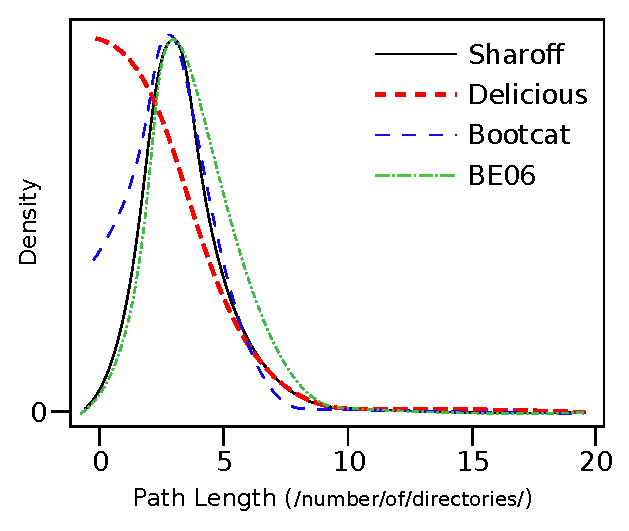
\includegraphics[width=0.8\textwidth]{longitudinal/attrition-density}
    \caption{Differences in the empirical distribution of URI path length.}
    \label{fig:longitudinal:attrition:attrition-density}
\end{figure}


% URI ARGUMENTS (dynamic-ness)
% SUMMARY OF ARGUMENTS
    %> summary(factor(be.s3$uri_nargs))
      %0   1   2   3   4 
    %353  58  47   6   1 
    %> summary(factor(deli.s3$uri_nargs))
	 %0      1      2      3      4      5      6      7      8      9     10 
    %579415  36137   8276   2445   1166    459    205    116     76     45     15 
	%11     12     13     14     15     16     17     19     29     30 
	%11     12     10      3      1      2      1      1      1      1 
    %> summary(factor(serge.s3$uri_nargs))
	%0     1     2     3     4     5     6     7     8     9 
    %68176  8637  2905  1434   458   202    65    12    19     2 
    %> summary(factor(boot.s3$uri_nargs))
	 %0      1      2      3      4      5      6      7      8      9     10 
    %165894   7339   2039    633    294    129     37     29      4     20     13 
	%11     12     15     18     20 
	 %1      3      1      1      1 
%ARGC > 0 COUNTS
    %> summary(factor(be.s3$uri_nargs > 0))
    %FALSE  TRUE 
      %353   112  = 23.68%
    %> summary(factor(deli.s3$uri_nargs > 0))
    %FALSE   TRUE  
    %579415  48983  = 8.45%
    %> summary(factor(serge.s3$uri_nargs > 0))
    %FALSE  TRUE 
    %68176 13734  = 16.70%
    %> summary(factor(boot.s3$uri_nargs > 0))
     %FALSE   TRUE 
    %165894  10544  = 5.95%
Taking the presence of GET-arguments in a URI 
as an indicator of a page being dynamic, a number of effects may be seen across the corpora.  The BE06 corpus had 24\% of all links dynamic, exceeding Sharoff's at 17\% and Delicious \& BootCat at 8\% and 6\% respectively.  This difference is probably due to the selection of published documents, since the compiler was seeking specific materials within sites rather than attempting to retain the location of a resource (as with Delicious) or sampling randomly from URI-space (as with BootCat).  Differences between the two BootCat-based corpora may reflect changing weights within search engine algorithms. %TODO: which may also use this property as an indicator, amongst other things











%--------------------------------------------------------------------------------

\subsection{Discussion}

% these next three bits may be better in the conclusion/future-work section
%In addition, the searching model for WaC samples language through search engine APIs which apply a lens of common usefulness in their modelling of search results. This lens represents a consumption-based sampling strategy, rather than one of production. This may also have implications for the WaC paradigm in terms of the resulting language sample.

%The decentralised architecture of the web has great implications for online content availability --- whereas some sites are large, publishing and holding content for authors, others constitute a single, self-published work.  The distinction between these is weak online, and, crucially, tied to the topic and purpose of the text itself.  

%It seems reasonable, for example, to state that news websites are generally more long-lived than personal or hobby websites, which are backed by individuals.  This attrition of documents online may cause skew in the representativeness of any samples taken from an open-source corpus, as well as producing a drift in any results computed from web-as-corpus studies (especially those with small sample sizes or specialised subject areas).


These preliminary results indicate that the process of corpus compilation, by introducing deliberate bias into the content  (the selection of full documents, filtering of navigation pages, etc.), impacts the observed document attrition rate.  These biases have been evidenced by the URI features alone, raising interesting questions about the effect that collection strategies have upon corpus integrity --- should the tendencies of different groups of web publishers be factored into sampling strategies for open-source or subject-specific corpora?

The ramifications of these biases for the WaC availability sampling strategy remain an open question --- does `searching' for links imply a minimum age, and hence a pre-existing skew towards certain content?

% rephrase? not sure about 'observe' and what you mean here
There are indications that sampling a cross-section of production, rather than consumption, observes the initial steep decline in document availability that is inherent in most survival distributions%( mention exponential vs bathtub shaped curve?, nope-SW)
.  It is possible that these effects are minimised by the WaC approach, and are actually more pronounced in conventional, offline, corpora: search-based sampling may compensate for this effect by weighting reliable and established websites through the algorithms used to rank relevance, though further work is needed to establish the degree to which this occurs.  Another possible effect is the disproportionate availability of archived, out of copyright, documents.


%These results hint at the scale of the bias applied when selecting documents online, relative to their longevity.  These biases seem to be explainable partially in terms of the findings of other web attrition studies, implying that the method of URI selection is key in discounting pages with dynamic or non-document content (such as navigation, help or launch pages).

%In the best case, where all linguistic areas decay at a similar rate, this merely causes us to question the validity of corpora sampled a short time ago.  Where conclusions depend upon the changing nature of presentation or context this change is likely to be more pronounced, as websites taken down are notionally unlikely to be uploaded without some degree of change.


% TODO: not compensating for server-side 404 error messages

% ------------- Vestigial notes -----------
%1) Different methods of building corpora represent different portions of the web in such a way that affects their longevity
%2) BE06-style sampling of \_production\_ rather than consumption online seems to cause high volatility (bathtub-shaped failure curve?)
%3) Long-term, high-resolution study necessary to idenfity patterns of loss over a year (clustered around tax year?)
%4) study limitations
%    * not compensating for server-generated pseudo-404 messages
%    * Not taking into account changing content/topic (or content at all)
%    * not taking into account role of page (navigation, etc)
%    * wildly heterogenous data sources due to availability sample




% -----------------------------------------------------------------------------
\subsubsection{Further Work}
Further sampling and analysis is necessary to confirm the issues highlighted above.  This paper comprises a preliminary look at data sampled in a longitudinal study, which will go on to relate the influences of extrinsic document features (which may be used to inform sampling strategies) to their linguistic content.  

This will involve, primarily, identifying the extent to which document attrition applies bias on linguistic content, rather than technical features, and how this varies through the sampling period.  Issues of particular interest include:

\begin{itemize}
    %\item The extent to which attrition online skews the linguistic content of corpora;%, and if this may be compensated for by careful construction;
    %\item The rate of change of documents online from a semantic, rather than technical, standpoint;
    \item The distribution through time of documents online --- does sampling using search engines apply particular topical bias as they respond to time-critical events?; % regular or lumpy, is this periodic? related to other stuff?
	\item The propensity of document contents to change in meaningful ways (rather than simply updating boilerplate and navigation page code);
    \item Whether similar documents or websites display similar levels of loss;
    \item The characteristics of compilation strategies with regards to their effects on attrition --- is it possible to control biases in web-derived corpora through stratified or two-phase sampling techniques.
\end{itemize}



% ------------- Vestigial notes -----------
% * Analysis of content relative to attrition
% * Analysis of change relative to attrition
% * Analysis of "threshing" and how it affects open source corpora
% * Analysis of the curve of death relative to content/change
% * Topic-distance vs attrition, create a [compensatory] model for topic-space (including nice 3D surface graphs)



